\documentclass[a4paper,12pt]{article}
\usepackage{amssymb} % needed for math
\usepackage{amsmath} % needed for math
\usepackage[utf8]{inputenc} % this is needed for german umlauts
\usepackage[ngerman]{babel} % this is needed for german umlauts
\usepackage[T1]{fontenc}    % this is needed for correct output of umlauts in pdf
\usepackage[margin=2.5cm]{geometry} %layout
\usepackage{booktabs}
\usepackage[hidelinks]{hyperref}
\hypersetup{pdftitle={Balanced Banana},bookmarks=true,}
\usepackage{graphicx}
\usepackage{csquotes}
\usepackage[nonumberlist]{glossaries}
\usepackage{enumitem}
\usepackage{verbatim}
\usepackage{indentfirst} % Adds indent for the first paragraph after a {/section}


\deftranslation[to=ngerman]{Glossary}{\section{Stichwortverzeichnis}}

\makeatletter
\newenvironment{mycode}
 {\def\@xobeysp{\ }\verbatim\rightskip=0pt plus 6em\relax}
 {\endverbatim}
\makeatother

\title{Balanced Banana}
\author{Niklas Lorenz \and Thomas Häuselmann \and Rakan Zeid Al Masri \and Christopher Lukas Homberger \and Jonas Seiler}


%%%%%%%%%%%%%%%%%%%%%%%%%%%%%%%%%%%%%%%%%%%%%%%%%%%%%%%%%%%%%%%%%%%%%%
% Create a shorter version for tables. DO NOT CHANGE               	 %
%%%%%%%%%%%%%%%%%%%%%%%%%%%%%%%%%%%%%%%%%%%%%%%%%%%%%%%%%%%%%%%%%%%%%%
\newcommand\addrow[2]{#1 &#2\\ }

\newcommand\addheading[2]{#1 &#2\\ \hline}
\newcommand\tabularhead{\begin{tabular}{lp{13cm}}
\hline
	}

\newcommand\addmulrow[2]{ \begin{minipage}[t][][t]{2.5cm}#1\end{minipage}%
   &\begin{minipage}[t][][t]{8cm}
    \begin{enumerate} #2   \end{enumerate}
    \end{minipage}\\ }

\newenvironment{usecase}{\tabularhead}
{\hline\end{tabular}}

\usepackage{microtype}

\begin{document}
\pagenumbering{roman}
\begin{titlepage}
    \begin{center}
    
     \vspace*{0.8cm}
 
        
\includegraphics[width=0.5\textwidth]{balancedbanana}
        \vspace*{1cm}
 
        \Huge
        \textbf{Balanced Banana}
 
        \vspace{0.5cm}
        \LARGE
        A Distributed Task Scheduling System
        
        \vspace{0.5 cm}
        \LARGE
        Pflichtenheft
 
        \vspace{1.5cm}

        \large
        \textbf{Niklas Lorenz, Thomas Häuselmann, Rakan Zeid Al Masri, Christopher Lukas Homberger und Jonas Seiler}
 
        \vspace*{0.5cm}

        \textbf{\today}
 
       
        
 
    \end{center}
\end{titlepage}         % Deckblatt.tex laden und einfügen
\setcounter{page}{2}
\tableofcontents          % Inhaltsverzeichnis ausgeben
\clearpage
\pagenumbering{arabic}

\section{Einleitung}
\vspace{0.2cm}
Dieses Dokument dient als Übersicht der Qualitätssicherung. Erläutert werden sowohl unsere Methoden zur Qualitätssicherung als auch das Ergebnis dieser. Ebenfalls beinhaltet dieses Dokument eine Anleitung zum Aufsetzen und Benutzen des endgültigen Programms.
\clearpage
\section{Testabdeckung}
\subsection{Klassenüberdeckung}
\vspace{0.2cm}
Die Testüberdeckung der einzelnen Klassen ist in der ersten Woche der Qualitätssicherung gefallen, dies liegt daran, dass einige Klassen zwar intern funktioneren, sie jedoch im Zusammenspiel mit anderen nicht. In der ersten Woche wurden also hauptsächlich fehlerhafte Schnittstellen oder andere Fehler beseitigt und entsprechende Unit Tests erst in den folgenden Wochen eingeführt. \newline
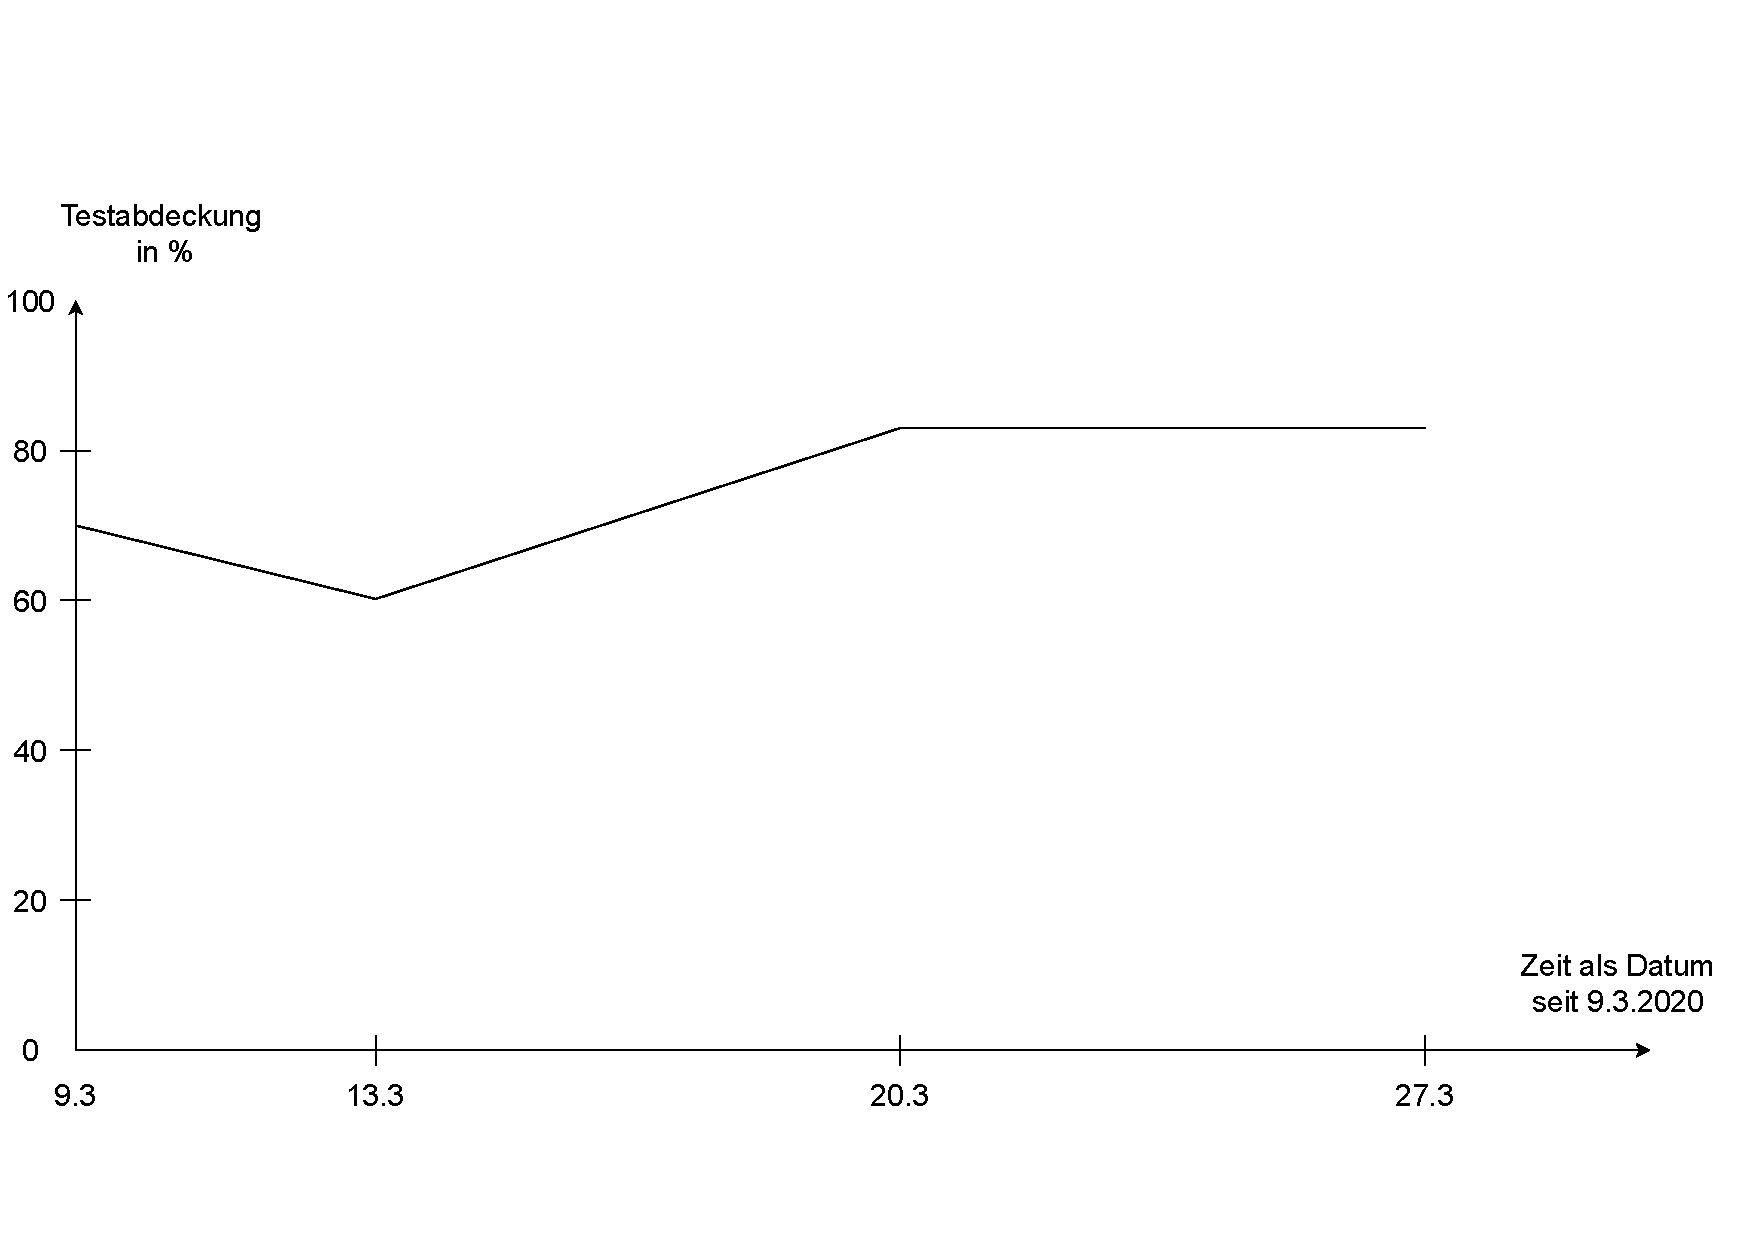
\includegraphics[width=\textwidth]{CoverageD} \newline
Entsprechend sehen wir einen Anstieg in Lines of Code (LOC) sowie der Anzahl Tests.
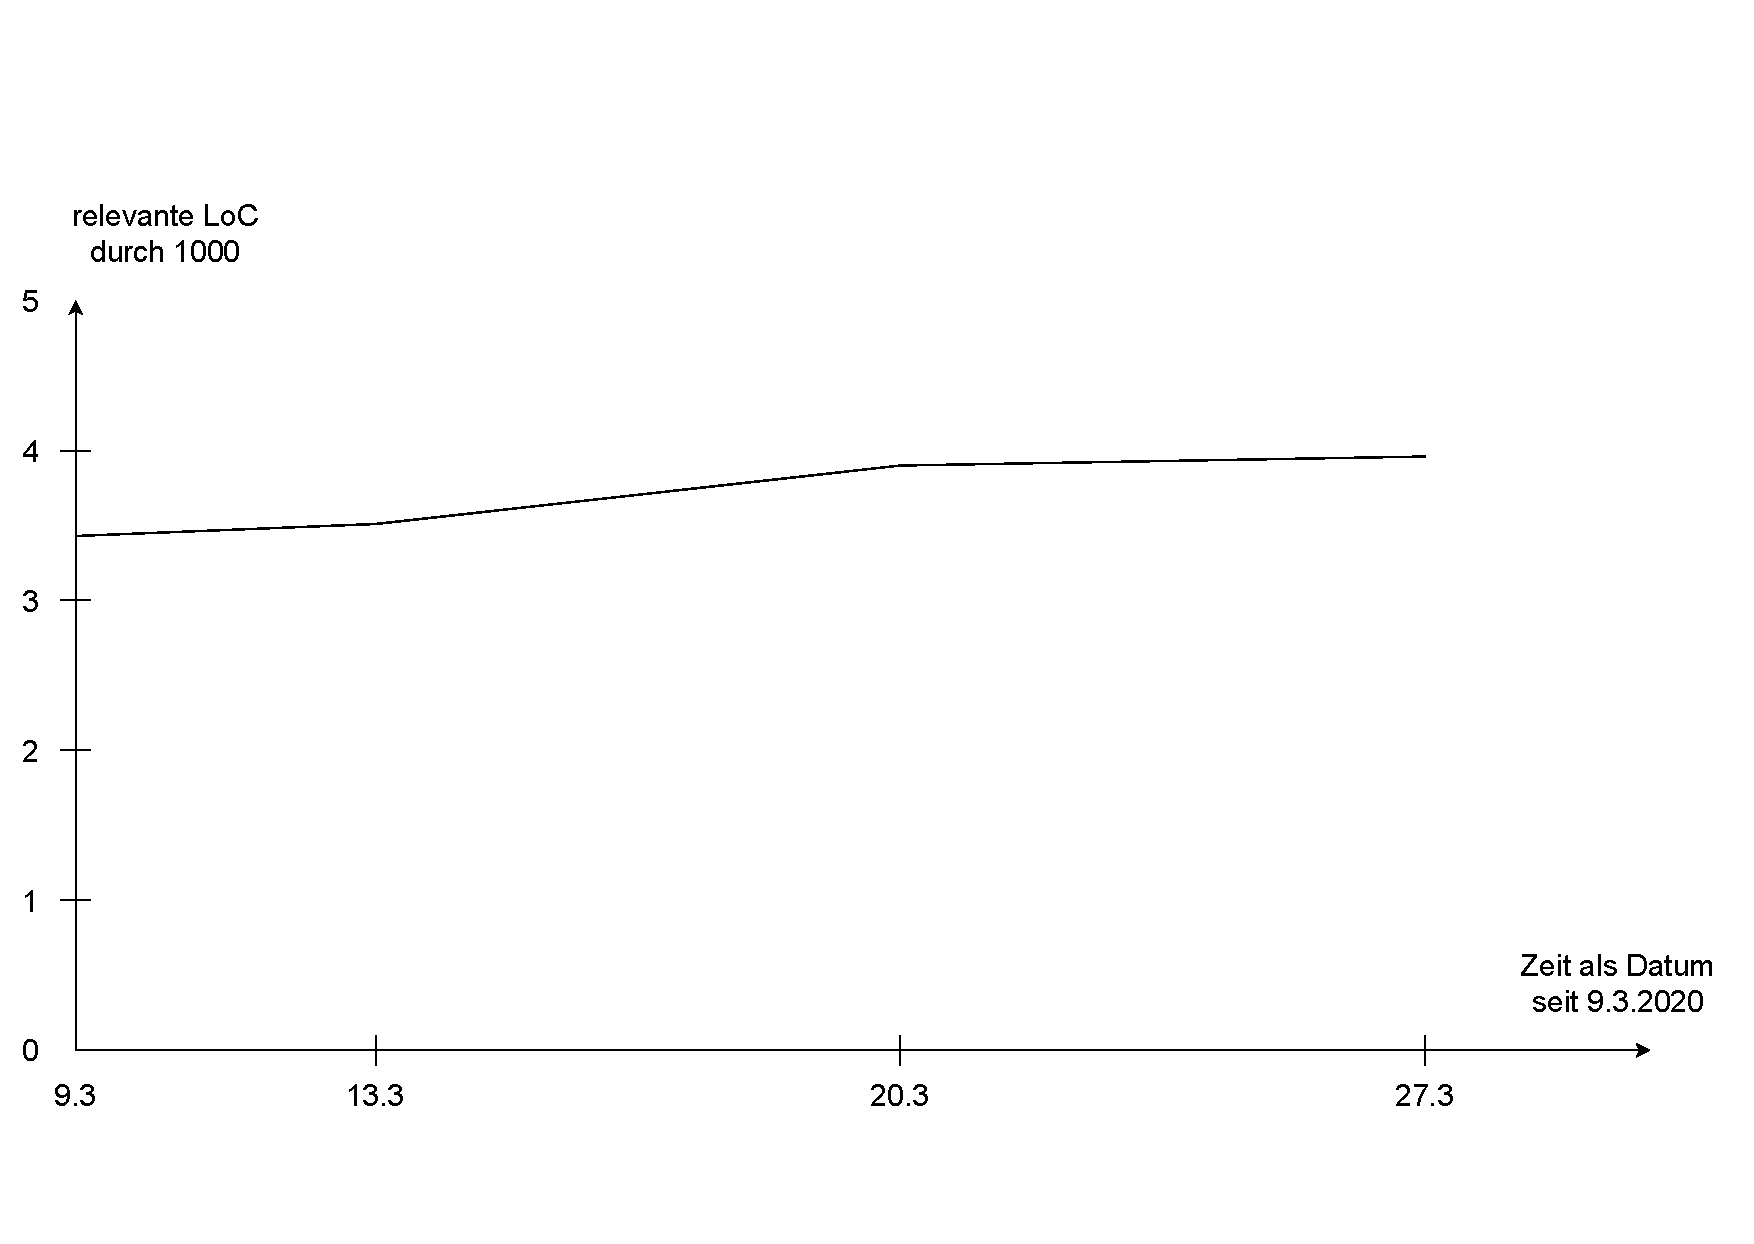
\includegraphics[width=\textwidth]{LOCD} \newline
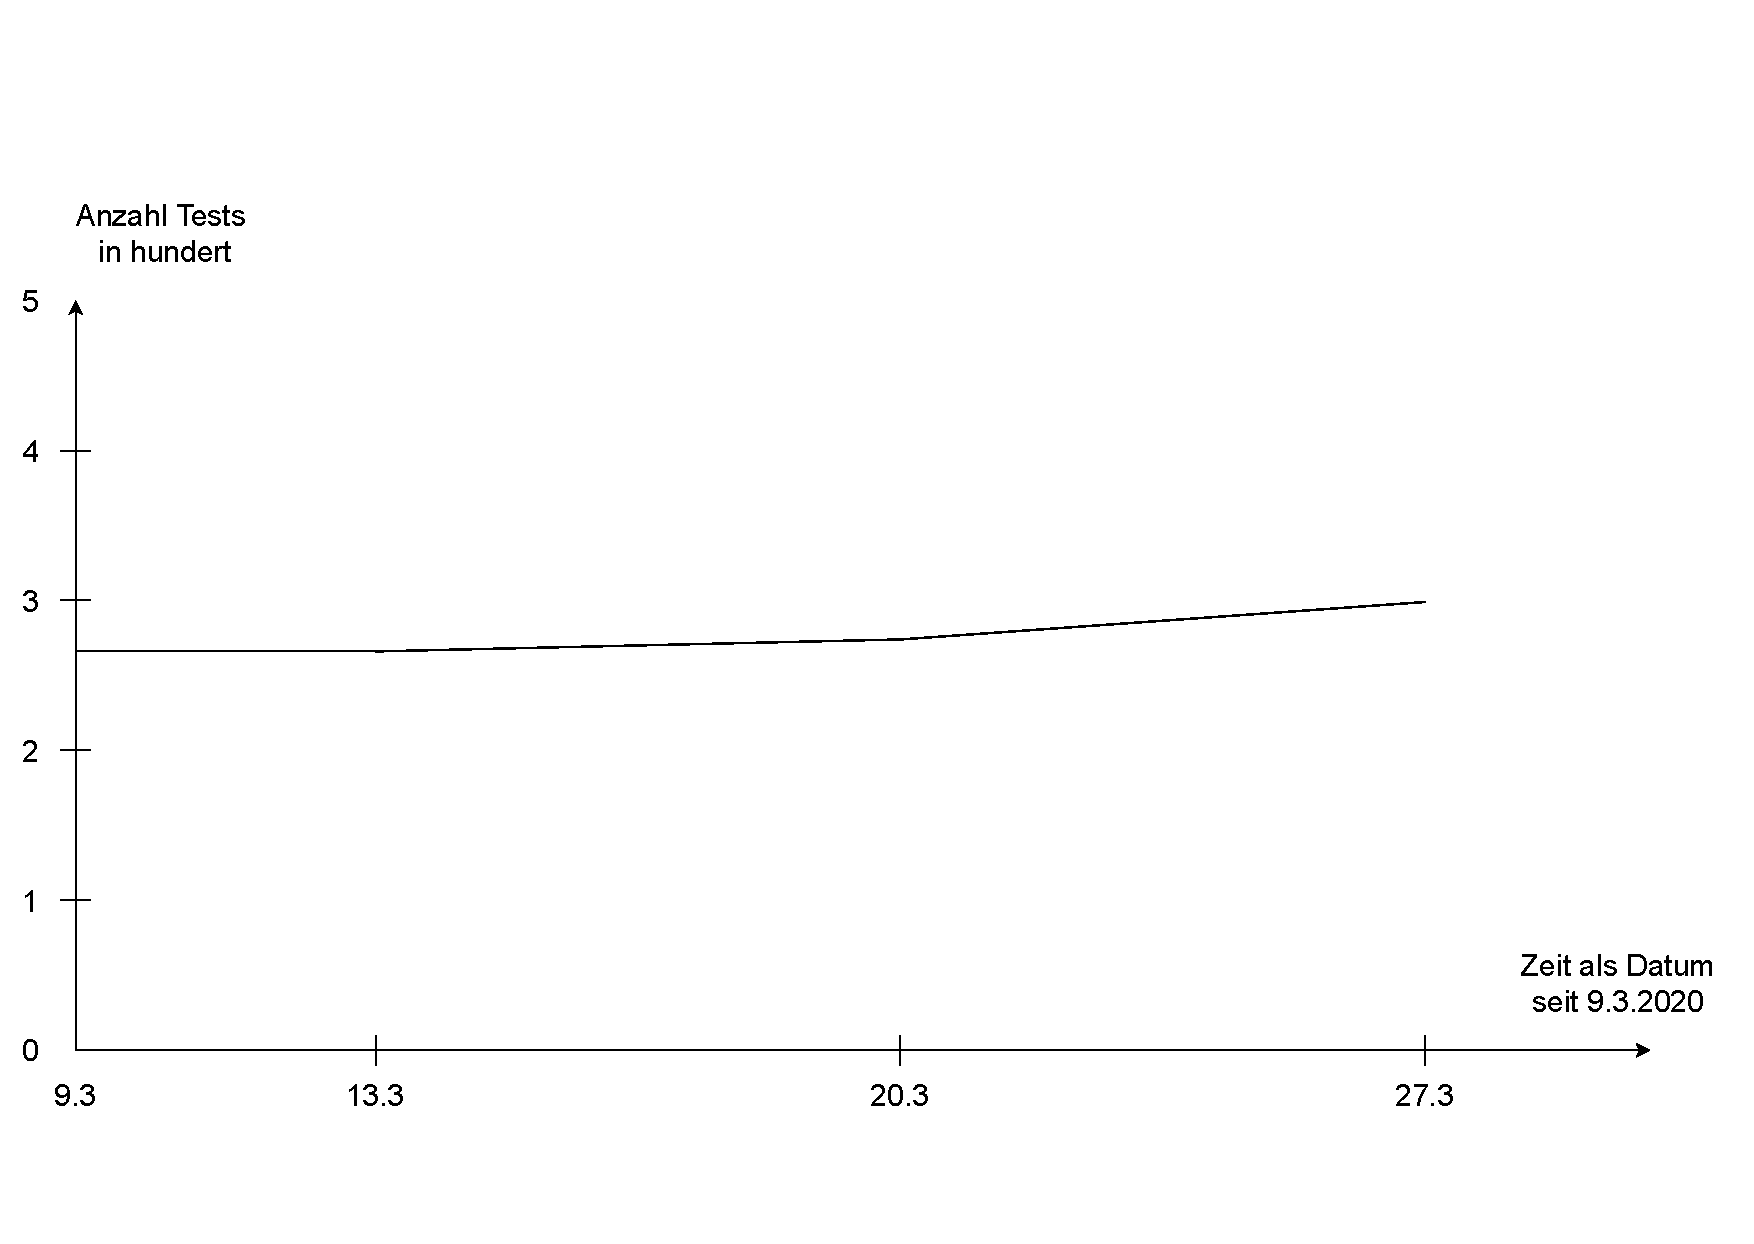
\includegraphics[width=\textwidth]{TestD} \newline
Da der Großteil des Codes bereits implementiert ist, sowie Integrationstests eher länger dafür aber weniger als Unittests sind, steigt auch die Anzahl der Tests nicht stark.
\clearpage
\subsection{Integrationstests}
\vspace{0.2cm}
Für das Automatisierte Testen des ganzen Systems haben wir ein Skript in Python benutzt, dieses beinhaltete diverse Szenarien und prüfte mit Positiv- als auch mit Negativtests. Neben diesem haben wir auch einiges "von Hand" getestet.
Die, im Pflichtenheft definierten, Testfälle werden wie folgt abgedeckt: \newline
\begin{tabular}{|l|c|r|}
	\hline
	T & Kurzbeschreibung & Wie getestet? \\ \hline \hline
	T1 & Verbinden des Clients mit Server & Automatisch \\ \hline
	T2 & Festlegen von Prioritäten & Manuell \\ \hline
	T3 & Festlegen des Betriebssystems & Manuell \\ \hline
	T4 & Abfragen eines Aufgabenstatus & Automatisch \\ \hline
	T5 & Benachrichtigung bei Abschluss einer Aufgaben & Manuell \\ \hline
	T6 & Erstellen von Sicherungen & Manuell \\ \hline
	T7 & Anforderung von Ausgabe & Manuell \\ \hline
	T8 & Abbrechen von zu langen Aufgaben & - \\ \hline
	T9 & Manuelles Stoppen von Aufgaben & Manuell \\ \hline
	T10 & Manuelle Sicherung von Aufgaben & Manuell \\ \hline
\end{tabular}
\newline \newline
In den Integrationstests haben wir hauptsächlich Verhalten getestet die so im Pflichtenheft noch nicht voraussagbar waren, daher haben wir tatsächlich mehr Tests als nur durch die vordefinierten ersichtlich.
\section{Umgesetzte Funktionale Anforderungen}

\begin{tabular}{|l|c|r|r|}
	\hline
	FA & Kurzbeschreibung & Implementiert? & Überdeckt von? \\ \hline \hline
	FA1 & Client verbindet sich mit Server & Ja & T1\\ \hline
	FA2 & Benutzer authentifiziert sich & Ja & Integrationstest\\ \hline
	FA3 & Benutzer kann Aufgaben einreihen & Ja & T2 \& T3\\ \hline
	FA4 & Benutzer kann Parameter übergeben & Ja & T2 \& T3\\ \hline
	FA41 & Client speichert Parameter in Config & Ja & Manuelltest\\ \hline
	FA42 & Benutzer kann Config übergeben & Ja & Manuelltest\\ \hline
	FA43 & Benutzer kann Priorität festlegen & Ja & T2\\ \hline
	FA44 & Benutzer kann min und max Cores festlegen & Ja & Manuelltest\\ \hline
	FA45 & Benutzer kann min und max RAM festlegen & Ja & Manuelltest\\ \hline
	FA46 & Benutzer kann Betriebssystem festlegen & Ja & T3\\ \hline
	FA47 & Benutzer kann angeben ob Client blockiert & Ja & Manuelltest\\ \hline
	FA48 & Benutzer übergibt Pfad zu Aufgabe & Ja & Integrationstest\\ \hline
	FA49 & Es können Standardwerte benutzt werden & Ja & Integrationstest\\ \hline
	FA5 & Benutzer kann Status von Aufgabe einsehen & Ja & T4\\ \hline
	FA6 & Benutzer bekommt Email bei Abschluss & Ja & T5 \\ \hline
	FA7 & Server erstellt Backups & (Nein) & T6 \\ \hline
	FA8 & Benutzer kann Ausgabe anfordern & Ja & T7\\ \hline
	FA9 & Benutzer kann Statistiken abfragen & Ja & Manuell\\ \hline \hline
	OFA1 & Benutzer kann Restzeit einsehen & Nein & - \\ \hline
	OFA2 & Server stoppt lange Aufgaben & Nein & T8 \\ \hline
	OFA3 & Benutzer kann manuell Aufgaben stoppen & Nein & T9 \\ \hline
	OFA4 & Benutzer kann manuell Aufgaben sichern & (Nein) & T10 \\ \hline
	OFA5 & Benutzer kann Pausierbarkeit angeben & (Nein) & - \\ \hline
\end{tabular}
\newline \newline
Für Anforderungen mit einem (Nein) existiert zwar in manchen Teilen des Programms die Funktionalität dafür, die Funktion selber ist jedoch nicht umgesetzt oder nutzbar.
\clearpage
\section{Benutzeranleitung}
\subsection{Aufsetzen des Schedulers}
\vspace{0.2cm}
Zuerst müssen wir das System aufsetzen, das Programm wird in einem Paket geliefert, die entsprechende Funktionen finden sich dann in den einzelnen ausführbaren Dateien.
\begin{itemize}[label={\textbullet}]
    \item Herunterladen des Programms unter\newline \texttt{https://github.com/balancedbanana/balancedbanana/releases}
    \item Einrichten der MySql Datenbank mit \newline
    \begin{mycode}
    cat balancedbanana.sql | sudo mysql
    \end{mycode}
    Die SQL Datei ist im Archiv unter \newline \texttt{share/balancedbanana/balancedbanana.sql} \newline
    zu finden.\newline
    Nun ist die Datenbank unter dem Schema balancedbanana installiert.
    In der MySQL-Konsole einen Datenbank Nutzer für balancedbanana anlegen mit folgenden MySQL-Befehlen:
    \begin{mycode}
    CREATE USER 'balancedbanana'@'localhost' IDENTIFIED BY 
    'balancedbanana';
    	
    GRANT ALL PRIVILEGES ON balancedbanana.* TO 'balancedbanana'@'localhost';
        
    FLUSH PRIVILEGES;
        
    exit
    \end{mycode}
    \item Configfiles pro Benutzer anlegen unter \newline
    \texttt{\$HOME/.bbc} bzw \texttt{.bbs} oder \texttt{.bbd}. \newline
    Dazu einfach die Configfiles von \newline
    \texttt{share/balancedbanana/.bbc} bzw \texttt{.bbs} oder \texttt{.bbd} \newline
    kopieren.
    \item  Das Passwort \texttt{balancedbanana} nach \texttt{IDENTIFIED BY} bei Bedarf anpassen und in \newline
    \texttt{\$HOME/.bbs/appconfig.ini} \newline
    in Zeile \texttt{databasepassword} anpassen. \newline
    
\end{itemize}
Nun ist der Scheduler aufgesetzt.
\subsection{Benutzen des Clients}
Der Client kann mit dem Programm \texttt{bbc} gestartet werden. Der Client hat verschiedene Subcommands sowie Flags für diese, nachführend sind diese erläutert. Für nicht angegebene Parameter wird zuerst in der Benutzerconfig (\texttt{\$HOME/.bbc}) dann in der Applikationsconfig (\texttt{share/balancedbanana/.bbc}) und danach wird entweder auf Standardwerte oder auf gesetzte Standardparameter im Scheduler gesetzt.
Bei Unklarheiten der Kommandos oder deren Parameter kann immer mit dem Argument -h ein Hilfemenü aufgerufen werden.
\subsubsection{Run}
Der Run-Command reiht eine Aufgabe ein, folgende Parameter sind verfübar:
\begin{itemize}
\item --server. Gibt die IP Adresse des Schedulers an. Angaben als String.
\item --port. Gibt den Port am Scheduler an. Angaben als 16 Bit Integer.	
\item --block / -b. Gibt an ob der Client blockiert, bis die Aufgabe beendet ist. Angaben als Boolean.
\item --email / -e. Gibt die Email an, die benachrichtigt wird, wenn die Aufgabe beendet ist. Angaben als String.
\item --image / -i. Gibt den Pfad des Images an, dass für die Aufgabe benutzt werden soll.  Angaben als String.
\item --priority / -p. Gibt die Priorität der Aufgabe an. Mögliche Werte sind "low","normal", "high".
\item --max-cpu-count / -C. Gibt die maximale Anzahl, der benutzten Kerne, der Aufgabe, an. Werte als 32 Bit Integer.
\item --min-cpu-count / -c. Gibt die minimale Anzahl, der benutzen Kerne, der Aufgabe, an. Werte als 32 Bit Integer.
\item --max-ram / -R. Gibt den maximal nutzbaren Arbeitsspeicher in miB an. Werte als 64 Bit Integer.
\item --min-ram / -r. Gibt den minimal nutzbaren Arbeitsspeicher in miB an. Werte als 64 Bit Integer.
\item --job / -j. Gibt die Eingabe an, die den Job startet. Alles hinter dieser Eingabe wird als Kommando aufgefasst, dieses Argument sollte also das letzte des Run Kommandos sein. Angaben als String.
\end{itemize}
Beispiel: \newline
\begin{mycode}
	./bbc run --server 192.168.178.82 --port 25565 -b true -e example@hello.com -i catsimulation -p high -C 4 -c 1 -R 4096 -r 1024 -j sh catsimulationfile.sh
\end{mycode}
\subsubsection{addImage}
Der addImage-Command registriert ein Image, sodass es mit --image eingereiht werden kann.
Das einzige Argument ist der Pfad zum Dockerfile.
Beispiel: \newline
\begin{mycode}
	./bbc addImage catsimulation ../../Simulations/Catsimulation	
\end{mycode}
\subsubsection{removeImage}
Entfernt ein registriertes Image unter dem gegebenen Namen. Das einzige Argument ist der Name des Images.
Beispiel: \newline
\begin{mycode}
	./bbc removeImage parrotsimulation
\end{mycode}
\subsubsection{status}
Frägt den Scheduler nach dem Status eines Jobs. Das einzige Argument ist die ID des Jobs als unsigned Integer. Beispiel: \newline
\begin{mycode}
	./bbc status 42
\end{mycode}
\subsubsection{tail}
Frägt den Scheduler nach den letzten ausgegebenen Zeilen der Aufgabe. Das einzige Argument ist die ID des Jobs als unsigned Integer. Beispiel: \newline
\begin{mycode}
	./bbc tail 42
\end{mycode}
\subsubsection{stop}
Stopt den angegebenen Job. Das einzige Argument ist die ID des Jobs als unsigned Integer. Beispiel: \newline
\begin{mycode}
	./bbc stop 43
\end{mycode}
\subsubsection{pause}
Pausiert den angegebenen Job. Das einzige Argument ist die ID des Jobs als unsigned Integer. Beispiel: \newline
\begin{mycode}
	./bbc pause 43
\end{mycode}
\subsubsection{continue}
Setzt den angegebenen Job fort. Das einzige Argument ist die ID des Jobs als unsigned Integer. Beispiel: \newline
\begin{mycode}
	./bbc continue 43
\end{mycode}
\subsubsection{backup}
Sichert den angegebenen Job. Das einzige Argument ist die ID des Jobs. Beispiel:
\newline 
\begin{mycode}
	./bbc backup 43
\end{mycode}
\subsubsection{restore}
Stellt den angegeben Job aus einem Backup wieder her. Das einzige Argument ist die Backup ID. Beispiel: \newline
\begin{mycode}
	./bbc restore 240
\end{mycode}
\subsection{Benutzen des Schedulers}
Der Scheduler hat im Gegensatz zum Client keine unterschiedlichen Kommandos und muss nur gestartet werden. Bei Unklarheiten kann wieder mit -h ein Hilfemenü aufgerufen werden. Folgende Parameter stehen zur Verfügung:
\begin{itemize}
	\item --server / -s. Legt fest auf welcher IP-Adresse der Scheduler gestartet wird. Angaben als String.
	\item --webapi / -w. Legt fest auf welcher IP-Adresse die WebAPI des Schedulers gestartet wird. Angaben als String.
	\item --serverport / -S. Legt fest auf welchem Port der Scheduler gestartet wird. Angaben als 32 Bit Integer.
	\item --webapi-port / -W. Legt fest auf welchem Port die WebAPI gestartet werden soll. Angaben als 32 Bit Integer
\end{itemize}
Hier ein Beispielaufruf:
\begin{mycode}
	./bbs -s 192.168.178.81 -w 192.168.178.82 -S 25565 -w 25566
\end{mycode}
\subsection{Benutzen des Workers}
Der Worker hat ebenfalls nur ein Kommando womit er gestartet wird. Bei Unklarheiten kann ebenfalls wieder mit -h ein Hilfemenü aufgerufen werden. Folgende Parameter stehen zur Verfügung:
\begin{itemize}
	\item --server / -s. Legt fest welche IP-Adresse der Scheduler hat. Angaben als String.
	\item --serverport / -S. Legt fest auf welchem Port der Scheduler gestartet wurde. Angaben als 32 Bit Integer.
\end{itemize}
Hier ein Beispielaufruf:
\begin{mycode}
	./bbd -s 192.168.178.82 -S 25565
\end{mycode}

\subsection{DevSetup}
Die Installationsanleitung für Entwickler, einschließlich einer Liste aller Pakete, Frameworks und Bibliotheken, sind unter \\
\texttt{https://github.com/balancedbanana/balancedbanana/blob/master/README.md} zu finden.
\section{Probleme und Bugs}
Die Phase der Qualitätssicherung wurde durch eine gewisse Pandemie gestört, daher fehlt uns eine richtige Testumgebung. Das Testen unter realen Umständen kam deshalb zu kurz oder gar nicht vor. Wir wissen aktuell noch nicht gut wie sich das Programm mit mehreren Workern verhält. \\ \newline \indent Ebenfalls haben wir zwar die Benachrichtigungsmails privat getestet, wissen jedoch nicht, ob diese fehlerfrei mit dem KIT-Mailserver funktionieren. \\ \newline \indent Die Anleitung zum Aufsetzen und Benutzen des Systems funktioniert auf unseren Systemen zwar, jedoch wissen wir nicht ob es auf den Systemen des CES zu anderweitigen Problemen kommen kann. \\ \newline
\indent Wir schätzen bei diesen Realtests noch einige Bugs zu finden, dies können wir jedoch aktuell nicht testen. \\
\newline
\indent Einige Funktionen, wie das Stoppen und Fortführen von Jobs, sind, wegen des experimentellen Checkpoint Features von Docker, in keinem konsistent ausführbaren Zustand. Das Aufsetzen der Funktionen ist kompliziert und deshalb haben wir die Funktion vorerst als implementiert aber nicht nutzbar angemerkt. \\
\newline
\indent Ein kleineres Problem ist das Beschreiben des RAMs. Beim Scheduler besteht die Chance, dass sich die Daten im Arbeitsspeicher festsetzen und diesen somit irgendwann vollschreiben. Wir empfehlen also, den Scheduler einmal alle paar Monate neu zu starten. \newline
\section{Konklusion}
Da die Qualitätssischerungsphase mit der Quarantäne kollidierte, fehlt uns leider Erfahrung mit der echten Benutzung des Systems. Trotzdem schafft unser Programm die von uns gestellten Szenarien. Viele optionale Features existieren ebenfalls als Funktion, wir empfehlen jedoch nicht diese aktuell zu benutzen. Wir denken, dass unser Programm an einem Punkt angekommen ist, an dem es mit realem Testen, und sukzessiven Beseitigen der Probleme, gut funktionieren sollte.
Zusammenfassend sind wir zufrieden mit dem Ergebnis.

\clearpage
\end{document}
